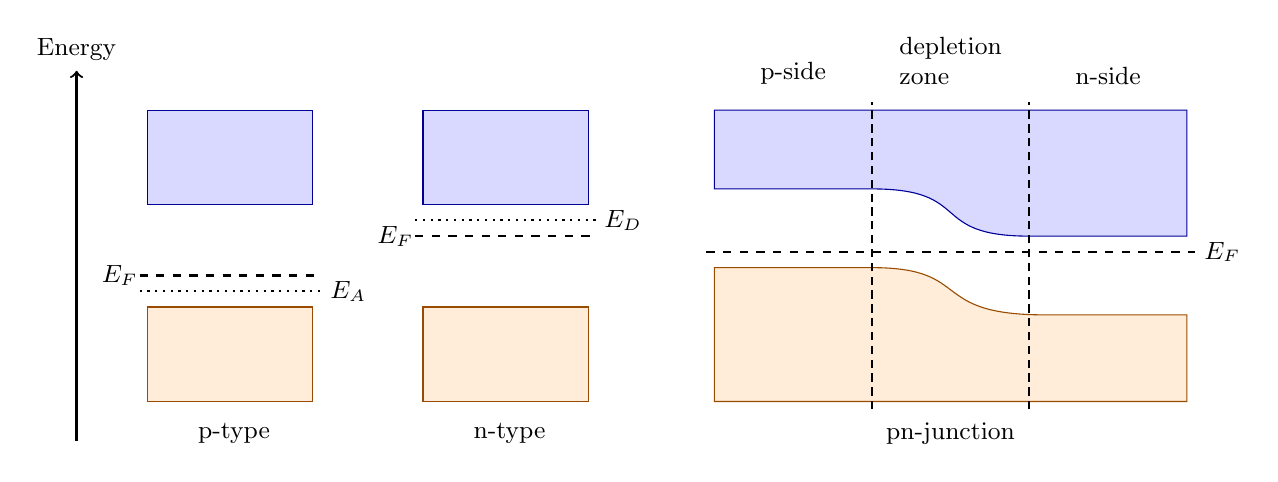
\begin{tikzpicture}[font=\small]
    
    % ── parameters ──────────────────────────────────────────────────
    \def\bw{2.2}   % band width
    
    % x-centres of the three columns
    \def\xIns{0}
    \def\xSemi{3.5}
    \def\xCond{8}
    
    
    % ── p-type ───────────────────────────────────────────────────
    \fill[orange!15] (-1.1, 0) rectangle (1, 1.2);
    \draw[orange!60!black] (-1.1, 0) rectangle (1, 1.2);
    
    \fill[blue!15] (-1.1, 2.5) rectangle (1, 3.7);
    \draw[blue!60!black] (-1.1, 2.5) rectangle (1, 3.7);
    
    \draw[dashed, thick] (-1.2, 1.6) -- (1.1, 1.6);
    \node[left] at (-1.1, 1.6) {$E_F$};
    
    \draw[dotted, thick] (-1.2, 1.4) -- (1.1, 1.4);
    \node[left] at (1.8, 1.4) {$E_A$};
    
    \node[below] at (\xIns, -0.15) {p-type};
    
    % ── n-type ───────────────────────────────────────────────
    \fill[orange!15] (-1.1+\xSemi, 0) rectangle (1+\xSemi, 1.2);
    \draw[orange!60!black] (-1.1+\xSemi, 0) rectangle (1+\xSemi, 1.2);
    
    \fill[blue!15] (-1.1+\xSemi, 2.5) rectangle (1+\xSemi, 3.7);
    \draw[blue!60!black] (-1.1+\xSemi, 2.5) rectangle (1+\xSemi, 3.7);
    
    \draw[dashed, thick] (-1.2+\xSemi, 2.1) -- (1.1+\xSemi, 2.1);
    \node[left] at (-1.1+\xSemi, 2.1) {$E_F$};
    
    \draw[dotted, thick] (-1.2+\xSemi, 2.3) -- (1.1+\xSemi, 2.3);
    \node[left] at (1.8+\xSemi, 2.3) {$E_D$};
    
    \node[below] at (\xSemi, -0.15) {n-type};
    
    % ── pn-junction ─────────────
\draw[fill=blue!15, draw=blue!60!black]
  (\xCond+4.1, 2.1) -- (\xCond+4.1, 3.7) -- (\xCond-1.9, 3.7) -- (\xCond-1.9, 2.7) -- (\xCond+0.1, 2.7)
  .. controls (\xCond+1.4, 2.7) and (\xCond+0.8, 2.1) ..
  (\xCond+2.1, 2.1) -- cycle;

\draw[fill=orange!15, draw=orange!60!black]
  (\xCond-1.9, 1.7) -- (\xCond-1.9, 0) -- (\xCond+4.1, 0) -- (\xCond+4.1, 1.1) -- (\xCond+2.3, 1.1)
  .. controls (\xCond+0.8, 1.1) and (\xCond+1.4, 1.7) ..
  (\xCond+0.1, 1.7) -- cycle;

\node[below] at (\xCond+1.1, -0.15) {pn-junction};
\node[above] at (\xCond-0.9, 3.9) {p-side};
\node[above, align=left] at (\xCond+1.1, 3.9) {depletion \\ zone};
\node[above] at (\xCond+3.1, 3.9) {n-side};
\draw[dashed, thick] (\xCond-2, 1.9) -- (\xCond+4.2, 1.9);
\node[right] at (\xCond+4.2, 1.9) {$E_F$};
\draw[densely dashed, thick] (\xCond+0.1, -0.1) -- (\xCond+0.1, 3.8);
\draw[densely dashed, thick] (\xCond+2.1, -0.1) -- (\xCond+2.1, 3.8);
    
    
    % ── ENERGY AXIS ──────────────────────────────────────────────────
    \draw[->, thick] (-2, -0.5) -- (-2, 4.2) node[above] {Energy};

\end{tikzpicture}